\subsection{Lagrange Polynomial Interpolation}
\label{theory-lagrange}

Below we present the theory of interpolation using \textit{Lagrange} polynomials, applied to simplex geometries, This section is inspired by \cite{koshiba+2000, ilic+2003, berrut+2004}, and is a summary of well-known results. The goal of \textit{Lagrange} interpolation is to construct a mapping $\vec{x} = \vec{p}(\vec{r})$ from local coordinates of an entity to global coordinates of the domain. In its own local coordinates, the entity will be denoted as a reference element \citeDune{}. A simplex reference element $\Delta_d$ of dimension $d$ is given by the following local coordinates:
%
\begin{table}[H]
\centering
\begin{tabular}{l l l}
\hline
  Label & Dimension & Coordinates \\ \hline
  $\Delta_0$ & 0 & $\{ 0 \}$ \\
  $\Delta_1$ & 1 & $\{ 0\}, \{ 1\}$ \\
  $\Delta_2$ & 2 & $\{ 0, 0 \}, \{ 1, 0 \}, \{ 0, 1 \}$ \\
  $\Delta_3$ & 3 & $\{ 0, 0, 0 \}, \{ 1, 0, 0 \}, \{ 0, 1, 0 \}, \{ 0, 0, 1 \}$
\end{tabular}
\caption{Reference element local coordinates}
\label{table:lagrange:refelement}
\end{table}
%
\noindent
Local simplex geometries can be parametrized using the local coordinate vector $\vec{r}$:
%
\begin{table}[H]
\centering
\begin{tabular}{l l l}
\hline
  Entity      & Parametrization    & Range \\ \hline
  Edge        & $\vec{r}=(u)$      & $u \in [0,1]$ \\
  Triangle    & $\vec{r}=(u,v)$    & $u \in [0,1]$ and $v \in [0, 1-u]$ \\
  Tetrahedron & $\vec{r}=(u,v,w)$  & $u \in [0,1]$, $v \in [0, 1-u]$ and $w \in [0, 1-u-v]$
\end{tabular}
\caption{Reference element parametrization in local coordinates}
\label{table:lagrange:parametrization}
\end{table}



%\paragraph{Interpolatory Vertices}
%\label{theory-lagrange-vertices}
\noindent
\textbf{Interpolatory Vertices}

\noindent
In order to define the curvilinear geometry, a set of global coordinates $\vec{x}_i = \vec{p}_i(\vec{r}_i)$, known as interpolatory vertices, is provided. By convention, the interpolatory vertices correspond to a sorted structured grid on a reference simplex, namely
\[\vec{r}_{i,j,k} = \frac{(k,j,i)}{Ord}, \;\;\; i=[0..Ord], \;\;\; j=[0..Ord-i], \;\;\; k=[0..Ord-i-j]\]
where $Ord$ is the interpolation order of the entity. It is useful to construct a bijective map from a structured local grid to the provided global coordinates. It is the job of the meshing software to ensure that the global geometry of an entity does is not self-intersecting, non-singular, and that its curvature is optimized for PDE convergence \cite{lenoir1986}. In general, a non-uniform local interpolatory grid should be used in order to minimize the effect of \textit{Runge} phenomenon \cite{runge1901}. It is not an issue for lower polynomial orders, and is the standard currently provided by the available meshing software, so we shall restrict our attention only to uniform interpolation grids. The number of interpolatory points on a uniform grid over the reference simplex is described by triangular/tetrahedral numbers \cref{table:lagrange:nvertex}. These numbers are conveniently also the numbers describing the total number $N_{Ord}$ of polynomially-complete monomials up to a given order:
%
\begin{table}[H]
\centering
\begin{tabular}{l l l l l l l}
\hline
  Entity \textbackslash Order & 1 & 2  & 3  & 4  & 5 & general \\ \hline
  Edge                        & 2 & 3  & 4  & 5  & 6 & $Ord+1$\\
  Triangle                    & 3 & 6  & 10 & 15 & 21 & $(Ord+1)(Ord+2)/2$\\
  Tetrahedron                 & 4 & 10 & 20 & 35 & 56 & $(Ord+1)(Ord+2)(Ord+3)/6$
\end{tabular}
\caption{Number of vertices in a uniform interpolatory grid over the reference simplex}
\label{table:lagrange:nvertex}
\end{table}





% \paragraph{Interpolatory Polynomials}
% \label{theory-lagrange-polynomials}
\noindent
\textbf{Interpolatory Polynomials}

\noindent
The number of interpolatory vertices $N_{Ord}$ given in \cref{table:lagrange:nvertex} exactly matches the total number of monomials necessary to construct a complete polynomial of order $Ord$ or less. It can be observed that the uniform simplex discretization exactly matches the binomial/trinomial simplex, also known as the Pascal's triangle, commonly used to visualize the complete monomial basis. We define the function $z^{(dim, i)}(\vec{u})$ as the set of all monomials of dimension $dim$ and order less than or equal to $i$. The first few sets for 1D, 2D and 3D are as follows:

\begin{flushleft}
\begin{table}[H]
\centering
\small
\begin{tabular}{l l l}
\hline
  Edge & Triangle & Tetrahedron \\ \hline
  
  
  \begin{minipage}[l]{0.34 \textwidth}
  \begin{eqnarray*}
	z^{(1,1)}(u) &=& \{1, u\}, \\
	z^{(1,2)}(u) &=& \{1, u, u^2\}, \\
	z^{(1,3)}(u) &=& \{1, u, u^2, u^3\}, \\
	z^{(1,4)}(u) &=& \{1, u, u^2, u^3, u^4\}, \\
	z^{(1,5)}(u) &=& \{1, u, u^2, u^3, u^4, u^5\},
  \end{eqnarray*}
  \; etc.
  \end{minipage} & 

  \begin{minipage}[l]{0.27 \textwidth}
  \begin{eqnarray*}
	z^{(2,1)}(u,v)	&=& \{1, u, v\}, \\
	z^{(2,2)}(u,v) &=& \{1, u, v, \\
	& & u^2, uv, v^2\},
  \end{eqnarray*}
  \; etc.
  \end{minipage} & 
  
  \begin{minipage}[l]{0.27 \textwidth}
  \begin{eqnarray*}
	z^{(3,1)}(u,v,w) &=& \{1, u, v, w\}, \\ 
	z^{(3,2)}(u,v,w) &=& \{1, u, v, w, \\
	& & u^2, uv, v^2, \\
	& & wu, wv, w^2\},
  \end{eqnarray*}
  \; etc.
  \end{minipage}
\end{tabular}
\normalsize
\caption{First few orders of the complete monomial basis for simplex entities }
\label{table:lagrange:monomial:function}
\end{table}
\end{flushleft}


\noindent
The mapping $\vec{p}(\vec{r})$ is chosen to exactly fit all the interpolatory vertices $\vec{x}_i$. Since the numbers of interpolatory vertices and monomials is the same, the interpolatory vertices will have a \textit{unique} associated \textit{complete} polynomial basis. This is not the same for entities of other geometry types. For example, for hexahedra, the above numbers do not match. Therefore, one either has to use a structured local grid with incomplete polynomial order basis, or choose a more sophisticated local discretization. Volakis et al \cite{volakis+2006} adopt the former approach, interpolating a 9 node 2\textsuperscript{nd} order rectangle with 4\textsuperscript{th} order incomplete polynomial basis that has a convenient separable tensor product form. \\

\noindent
One way to formulate the local-to-global coordinate mapping is
\begin{equation}
	\vec{p}(\vec{r}) = \sum_j L_j(\vec{r})\vec{x}_j 
\end{equation}
\noindent
where $\vec{p}_j $ are the fixed interpolatory vertices, and $L_j$ are the \textit{Lagrange} polynomials, defined by their interpolatory property
\begin{equation}
	\label{equation-lagrangepol-interpolatory-property}
	L_j(\vec{r}_i) = \delta_{ij}
\end{equation}
\noindent
for all local interpolatory vertices $\vec{r}_i$. The advantage of this formulation is that the \textit{Lagrange} polynomials are independent of the interpolatory vertices $\vec{x}_i$, and thus can be pre-computed and reused for all entities of a given order. It remains to determine the exact form of \textit{Lagrange} polynomials. We will present a short proof that \cref{equation-lagrangepol-basis-link} holds
\begin{equation}
	\label{equation-lagrangepol-basis-link}
	z_i(\vec{r}) = \sum_j L_j(\vec{r}) z_i (\vec{r}_j) 
\end{equation}
\noindent
Here, $\{z\}$ is a vector of monomials as defined in \cref{table:lagrange:monomial:function}. Given a fixed dimension $dim$, \cref{equation-lagrangepol-basis-link} should hold for all polynomial orders $Ord$. Both sides of \cref{equation-lagrangepol-basis-link} are polynomials of order at most $Ord$, which means that they have at most $N_{Ord}$ free parameters. Therefore, to prove that \cref{equation-lagrangepol-basis-link} holds in general, it is sufficient to show that it holds for $N_{Ord}$ different arguments. Thus, it is enough to show that it holds for all $\vec{r} = \vec{r}_k$, which in turn is true due to \cref{equation-lagrangepol-interpolatory-property}. Finally, we can combine all monomials and \textit{Lagrange} polynomials into corresponding vectors
\begin{equation}
	\vec{z} (\vec{r}) = V \vec{L} (\vec{r})
\end{equation}
\noindent
where $V_{ij} = z_i (\vec{r}_j)$, and find the \textit{Lagrange} polynomial coefficients by solving the linear system
\begin{equation}
	\label{equation-lagrange-linear-system}
	\vec{L} (\vec{r}) = V^{-1} \vec{z} (\vec{r})
\end{equation}

\noindent
It is important to note that the resulting interpolated geometry in global coordinates is not completely defined by the shape of its boundary, as the entire volume of the geometry inside the entity undergoes this polynomial transformation. \\


% \paragraph{Implementation for Simplices}
% \label{subsection-simplexgrid}
\noindent
\textbf{Implementation for Simplices}

\noindent
In this section we discuss how to efficiently enumerate the simplex interpolatory points and to construct the reference simplex grid. \\

\noindent
Let us define a simplex $\Delta^{\dim}_{n}$ of integer side length $n$, and place a set of points $\vec{\eta} \in \mathbb{Z}^{\dim}$ at unit intervals. This can be done by using nested loops
\begin{itemize}
	\item $\Delta^{1}_n = \{(i)\}$, for $i = [1$ to $n]$
	\item $\Delta^{2}_n = \{(j,i)\}$, for $i = [1$ to $n]$, $j = [1$ to $n - i]$
	\item $\Delta^{3}_n = \{(k,j,i)\}$, for $i = [1$ to $n]$, $j = [1$ to $n - i]$, $k = [1$ to $n - i - j]$
\end{itemize}

\noindent
Then, each integer vertex $(\Delta^{d}_n)_i$ corresponds exactly to the power of $u,v,w$ in the expansion of
\[ (1 + u)^n = \sum_{i=0}^n C^{(\Delta^{1}_n)_i}_n u^{(\Delta^{1}_n)_{i,1}} \]
\[ (1 + u + v)^n = \sum_{i=0}^n C^{(\Delta^{1}_n)_i}_n u^{(\Delta^{1}_n)_{i,1}} v^{(\Delta^{1}_n)_{i,2}} \]
\[ (1 + u + v + w)^n = \sum_{i=0}^n C^{(\Delta^{1}_n)_i}_n u^{(\Delta^{1}_n)_{i,1}} v^{(\Delta^{1}_n)_{i,2}} w^{(\Delta^{1}_n)_{i,3}} \]

\noindent
where $C^{i}_n, C^{i,j}_n$ and $C^{i,j,k}_n$ are the binomial, trinomial and quatrinomial coefficients. The powers of the parameters given in the above expansion correspond to the complete monomial basis for a polynomial of order $d$. The local coordinates of the uniform grid over the reference simplex can then be written as $r_i = \frac{1}{n}(\Delta^{d}_n)_i$ (see \cref{fig:lagrange:enumerationconstruction})

\begin{figure}[hp]
    \centering
    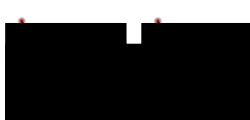
\includegraphics[scale=2.0]{images/curvilinear-numbering-generation}
    \caption{Construction of the uniform grid interpolatory points (right) from the \textit{Cartesian} coordinate enumeration}
    \label{fig:lagrange:enumerationconstruction}
\end{figure}

\noindent
After the monomials and the parametric interpolation points have been constructed, it remains to construct the interpolation matrix $V$ by evaluating the monomials at the interpolation points and to solve the linear system \cref{equation-lagrange-linear-system}, obtaining the \textit{Lagrange} polynomials. This has been implemented both explicitly, calculating and hard-coding all the simplex \textit{Lagrange} interpolatory polynomials, and implicitly, implementing symbolic polynomial arithmetic. The latter has the advantage of unrestricted polynomial order, as well as the freedom of further analytic manipulation using of symbolic arithmetic and explicit differential operators, but comes at the cost of slight computational overhead. \\

\noindent
The optimization of \textit{Lagrange} polynomial evaluation is of crucial importance, since they are typically evaluated a significant amount of times, especially during the integration and minimization procedures. Our implementation of \textit{Lagrange} polynomials benefits from the following observations:
\begin{itemize}
  \item Each \textit{Lagrange} polynomial of a given order uses the same monomial summands. It is thus of an advantage to evaluate all the \textit{Lagrange} polynomials at the same time, first evaluating all the necessary monomials, and then re-using the evaluated monomials to compute the polynomials.
  \item Along the same lines, evaluating all monomials of a given order at the same time is cheaper than evaluating them separately. Lower order monomials can be used to construct higher order monomials by doing a single multiplication per monomial.
\end{itemize}





